\chapter{连续函数}

本章将研究分析的拓扑基础, 并给出其初步应用. 我们主要将讨论限制在度量空间的拓扑上, 因为度量空间理论构成了分析学大部分内容的框架, 同时又足够简单和具体, 能最大限度地降低初学者的理解难度. 尽管如此, 度量空间的概念对于更深入的数学研究来说仍不够一般化, 因此, 在可能的情况下, 我们会给出在一般拓扑空间中同样成立的证明. 每一节的末尾都会讨论这些定理在一般拓扑空间中成立到何种程度. 这些讨论在初次阅读本书时可以略过, 但它们为读者提供了进入抽象拓扑的一个引导.

在第 1 节中, 我们考察度量空间之间的连续函数. 特别地, 我们将利用前一章中关于收敛序列的结果来研究连续性.

第 2 节专门讨论开集的概念. 其中一个关键结论是将连续函数刻画为具有 ``每个开集的原像仍为开集'' 性质的函数.

在接下来的一节中, 我们讨论紧度量空间. 尤其是, 我们将证明对于度量空间而言, 紧性与序列紧性是等价的. 紧性的重要性在本节所呈现的应用中已充分显现. 例如, 利用紧度量空间上连续实值函数的极值定理, 我们将证明 \(\K^n\) 上的所有范数均等价, 并给出代数基本定理的一个证明.

在第 4 节中, 我们研究连通空间与道路连通空间. 特别的, 我们将证明对于赋范向量空间的开子集, 这两个概念是一致的. 作为连通性的一个重要应用, 我们将证明介值定理的推广形式.

在这一段对抽象拓扑的简要探讨, 并为后续各章中的分析研究奠定基础之后, 本章剩余的两节转而研究实函数. 在简短的第 5 节中, 我们讨论实变量单调函数的性质, 并特别证明连续单调函数的反函数定理.

与本章前五节相对抽象的内容不同, 在最后一节这相对较长的部分中, 我们将学习指数函数及其相关函数: 对数函数、幂函数和三角函数. 在这部分研究中, 我们几乎运用了本章中引入的所有方法和定理.

\newpage

\section{连续性}

经验表明, 尽管函数通常可能非常复杂且难以描述, 但实际应用中出现的函数往往具有某些重要的定性性质, 其中之一便是连续性. 对于一个函数 \(f \colon X \to Y\), 其是否连续反映了像集 \(f(X) \subseteq Y\) 中的 ``微小变化'' 是如何由定义域 \(X\) 中相应的 ``微小变化'' 引起的. 为了使这一说法有意义, 必须为集合 \(X\) 和 \(Y\) 赋予某种额外的结构, 以便为 ``微小变化'' 提供精确的含义. 度量空间正是具备这种额外结构的显然候选者.

\subsection{基本性质与例子}

\begin{definition}[连续性]
    设 \(f \colon X \to Y\) 是度量空间 \((X, d_X)\) 和 \((Y, d_Y)\) 之间的函数. 称 \(f\) 在 \(x_0 \in X\) 处连续, 若对于任意 \(f(x_0)\) 的邻域 \(V \subseteq Y\) 存在 \(x_0\) 的邻域 \(U \subseteq X\) 使得 \(f(U) \subseteq V\). 并称 \(f\) 在 \(x_0\) 处不连续, 若 \(f\) 不在 \(x_0\) 处连续.
    \begin{center}
        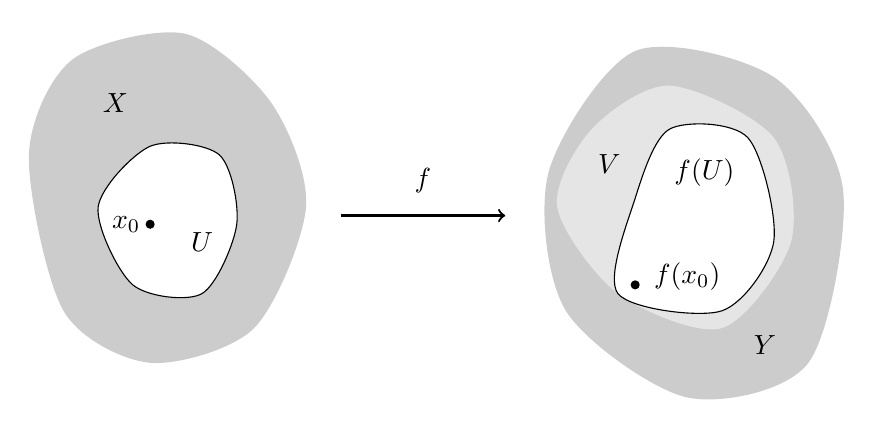
\begin{tikzpicture}[scale=1.1]
            % ---------- X ----------
            \draw[fill=gray!40, draw=none]
                plot[smooth cycle]
                coordinates {
                (-4,1.2) (-3.5,2.3) (-2.2,2.6) (-1.2,1.8)
                (-0.8,0.6) (-1.4,-0.8) (-2.6,-1.2)
                (-3.6,-0.6)
                };
            \node at (-3,1.8) {\(X\)};
            % ---------- U ----------
            \draw[fill=white, draw=black]
            plot[smooth cycle]
                coordinates {
                (-3.2,0.6) (-2.6,1.3) (-1.8,1.2)
                (-1.6,0.4) (-2.0,-0.4) (-2.8,-0.3)
                };
            \node at (-2,0.2) {\(U\)};
            % ---------- x0 ----------
            \fill (-2.6,0.4) circle (1.5pt);
            \node[left] at (-2.6,0.4) {\(x_0\)};
            % ---------- f ----------
            \draw[->, thick] (-0.4,0.5) -- (1.5,0.5);
            \node at (0.55,0.9) {\(f\)};
            % ---------- Y ----------
            \draw[fill=gray!40, draw=none]
                plot[smooth cycle]
                coordinates {
                (2.0,1.0) (3.0,2.4) (4.6,2.1)
                (5.4,0.8) (5.0,-1.2)
                (3.6,-1.6) (2.2,-0.6)
                };
            \node at (4.5,-1) {\(Y\)};
            % ---------- V ----------
            \draw[fill=gray!20, draw=none]
                plot[smooth cycle]
                coordinates {
                (2.1,0.6) (2.5,1.5) (3.4,2)
                (4.6,1.4) (4.8,0.2)
                (4.0,-0.8) (2.8,-0.4)
                };
            \node at (2.7,1.1) {\(V\)};
            % ---------- f(U) ----------
            \draw[fill=white, draw=black]
                plot[smooth cycle]
                coordinates {
                (3,0.7) (3.4,1.5) (4.3,1.4)
                (4.6,0.2) (4.0,-0.6)
                (2.8,-0.4)
                };
            \node at (3.8,1) {\(f(U)\)};
            % ---------- f(x0) ----------
            \fill (3,-0.3) circle (1.5pt);
            \node at (3.6,-0.2) {\(f(x_0)\)};
        \end{tikzpicture}
    \end{center}
    进一步, 称 \(f\) 是连续的, 若 \(f\) 在 \(X\) 中的每一点处都连续. 并称 \(f\) 是不连续的, 若 \(f\) 在 \(X\) 中至少一点处不连续. 最后, 将从 \(X\) 到 \(Y\) 的连续函数的全体记作
    \[
        C(X, Y) \coloneqq \{\, f \in Y^X \;;\; f\ \text{连续} \,\}\ .
    \]
\end{definition}

因此要证明 \(f\) 在 \(x_0\) 处连续, 应该假设给定 \(f(x_0)\) 的任意邻域 \(V\), 然后证明存在 \(x_0\) 的邻域 \(U\) 使得 \(f(U) \subseteq V\), 即对于任意 \(x \in U\) 都有 \(f(x) \in V\).

连续性的定义使用了邻域的概念, 因而相当简单. 但在具体问题中, 以下等价刻画往往更为实用.

\begin{proposition}
    度量空间之间的函数 \(f \colon X \to Y\) 在 \(x_0 \in X\) 处连续, 当且仅当对于任意 \(\varepsilon > 0\) 存在 \(\delta > 0\) 使得
    \[
        d_Y \bigl(f(x), f(x_0)\bigr) < \varepsilon\ ,\quad  x \in X\ \text{且}\ d_X(x, x_0) < \delta\ .
    \]
\end{proposition}

\begin{proof}
    \(\implies\). 假设 \(f\) 在 \(x_0\) 处连续. 任取 \(\varepsilon > 0\). 于是对于邻域 \(\B \bigl(f(x_0), \varepsilon\bigr) \in \nbr \big(f(x_0)\big)\) 存在 \(U \in \nbr(x_0)\) 使得 \(f(U) \subseteq \B \bigl(f(x_0), \varepsilon\bigr)\). 由邻域的定义可知存在 \(\delta > 0\) 使得 \(\B(x_0, \delta) \subseteq U\), 因此
    \[
        f \bigl(\B(x_0, \delta)\bigr) \subseteq f(U) \subseteq \B \bigl(f(x_0), \varepsilon\bigr)\ ,
    \]
    即当 \(d_X(x, x_0) < \delta\) 时 \(d_Y \bigl(f(x), f(x_0)\bigr) < \varepsilon\).

    \(\impliedby\). 假设对于任意 \(\varepsilon > 0\) 存在 \(\delta > 0\) 使得当 \(d_X(x, x_0) < \delta\) 时 \(d_Y \bigl(f(x), f(x_0)\bigr) < \varepsilon\). 任取 \(V \in \nbr \big(f(x_0)\big)\). 于是存在 \(\varepsilon > 0\) 使得 \(\B \bigl(f(x_0), \varepsilon\bigr) \subseteq V\). 由假设可知, 存在 \(\delta > 0\) 使得
    \[
        f \bigl(\B(x_0, \delta)\bigr) \subseteq \B \bigl(f(x_0), \varepsilon\bigr) \subseteq V\ ,
    \]
    因此 \(f\) 在 \(x_0\) 处连续.
\end{proof}

\begin{corollary}
    赋范向量空间之间的函数 \(f \colon X \subseteq E \to F\) 在 \(x_0 \in X\) 处连续, 当且仅当对于任意 \(\varepsilon > 0\) 存在 \(\delta > 0\) 使得
    \[
        \|f(x) - f(x_0)\|_F < \varepsilon\ ,\quad x \in X\ \text{且}\ \|x - x_0\|_E < \delta\ .
    \]
\end{corollary}

\begin{proof}
    由范数诱导的度量立刻可得.
\end{proof}

设 \(E \coloneqq F \coloneqq \R\), 函数 \(f \colon X \subseteq E \to F\) 由如下图像给出.
\begin{center}
    \begin{tikzpicture}
        % \draw (0,0) grid (8,5);
        % ================= 坐标轴 =================
        \draw[->] (-2,0) -- (8,0) node[right] {\(E = \R\)};
        \draw[->] (0,-1) -- (0,5) node[above] {\(F = \R\)};
        % ================= f =================
        \draw[thick] (-2,0.5) .. controls (-0.5,-1) .. (1.5,0.5);
        \draw[thick] (1.5,1.5) .. controls (3.5,3) and (5.5,2) .. (7.5,4.5) node[right] {\(f\)};
        % ================= x0 f(x0) =================
        \draw (5.6,3) -- (5.6,0) node[below] {\(x_0\)};
        \draw (5.6,3) -- (0,3) node[left] {\(f(x_0)\)};
        \draw[dashed] (4,2.5) -- (4,0) node[below] {\(x_0 - \delta\)};
        \draw[dashed] (4,2.5) -- (0,2.5);
        \draw[dashed] (7.2,4.1) -- (7.2,0) node[below] {\(x_0 + \delta\)};
        \draw[dashed] (7.2,4.1) -- (0,4.1) node[left] {\(f(x_0) + \varepsilon\)};
        \draw[dashed] (2.1,1.9) -- (2.1,0);
        \draw[dashed] (2.1,1.9) -- (0,1.9) node[left] {\(f(x_0) - \varepsilon\)};

        \draw (4,-0.9) -- (4,-1.1);
        \draw (7.2,-0.9) -- (7.2,-1.1);
        \draw (4,-1) -- (7.2,-1);
        \node at (5.6,-1.35) {\(U\)};

        \draw (-2.3,4.1) -- (-2.1,4.1);
        \draw (-2.3,2.5) -- (-2.1,2.5);
        \draw (-2.2,4.1) -- (-2.2,2.5);
        \draw[dashed] (0,2.5) -- (-2,2.5);
        \node at (-2.8,3.3) {\(f(U)\)};

        \draw (-3.8,4.1) -- (-3.6,4.1);
        \draw (-3.8,1.9) -- (-3.6,1.9);
        \draw (-3.7,4.1) -- (-3.7,1.9);
        \draw[dashed] (-1.8,1.9) -- (-3.7,1.9);
        \node at (-4.05,3) {\(V\)};

        % ================= x1 f(x1) =================
        \draw (1.5,0.5) -- (1.5,0) node[below] {\(x_1\)};
        \draw (1.5,0.5) -- (0,0.5) node[left] {\(f(x_1)\)};
        \draw (0.1,1.2) -- (-0.1,1.2) node[left] {\(f(x_1) + \varepsilon_1\)};
    \end{tikzpicture}
\end{center}
则 \(f\) 在 \(x_0\) 处连续, 这是因为对于任意 \(\varepsilon > 0\) 存在 \(\delta > 0\) 使得 \(U \coloneqq (x_0 - \delta, x_0 + \delta)\) 的像 \(f(U) \subseteq V \coloneqq \bigl(f(x_0) - \varepsilon, f(x_0) + \varepsilon\bigr)\). 另一方面, 不存在 \(\delta > 0\) 使得对于任意 \(x \in (x_1, x_1 + \delta)\) 都有 \(|f(x) - f(x_1)| < \varepsilon_1\), 因此 \(f\) 在 \(x_1\) 处不连续.